\documentclass[UTF8]{ctexart}

\usepackage{graphicx}

\title{铁磁共振实验报告}
\author{刘子安 PB20000069}

\begin{document}
\maketitle

\subsection{计算微波信号频率}

波长的平均值
$$\bar{\lambda} = \sum_{i=1}^{6}\lambda_i=\frac{3.162+3.161+3.163+3.161+3.163+3.162}{6}mm=3.162mm $$
根据刻度值和频率对照表可以求得微波信号频率
$$ \omega_0=\omega=895.3MHz$$

\subsection{计算$\Delta B$ 和 $g$ 因子}
我们从表中得出磁感应强度,并绘制出第一条$B$从小到大的$I-B$曲线: 

\begin{figure}[htbp]
	\centering
	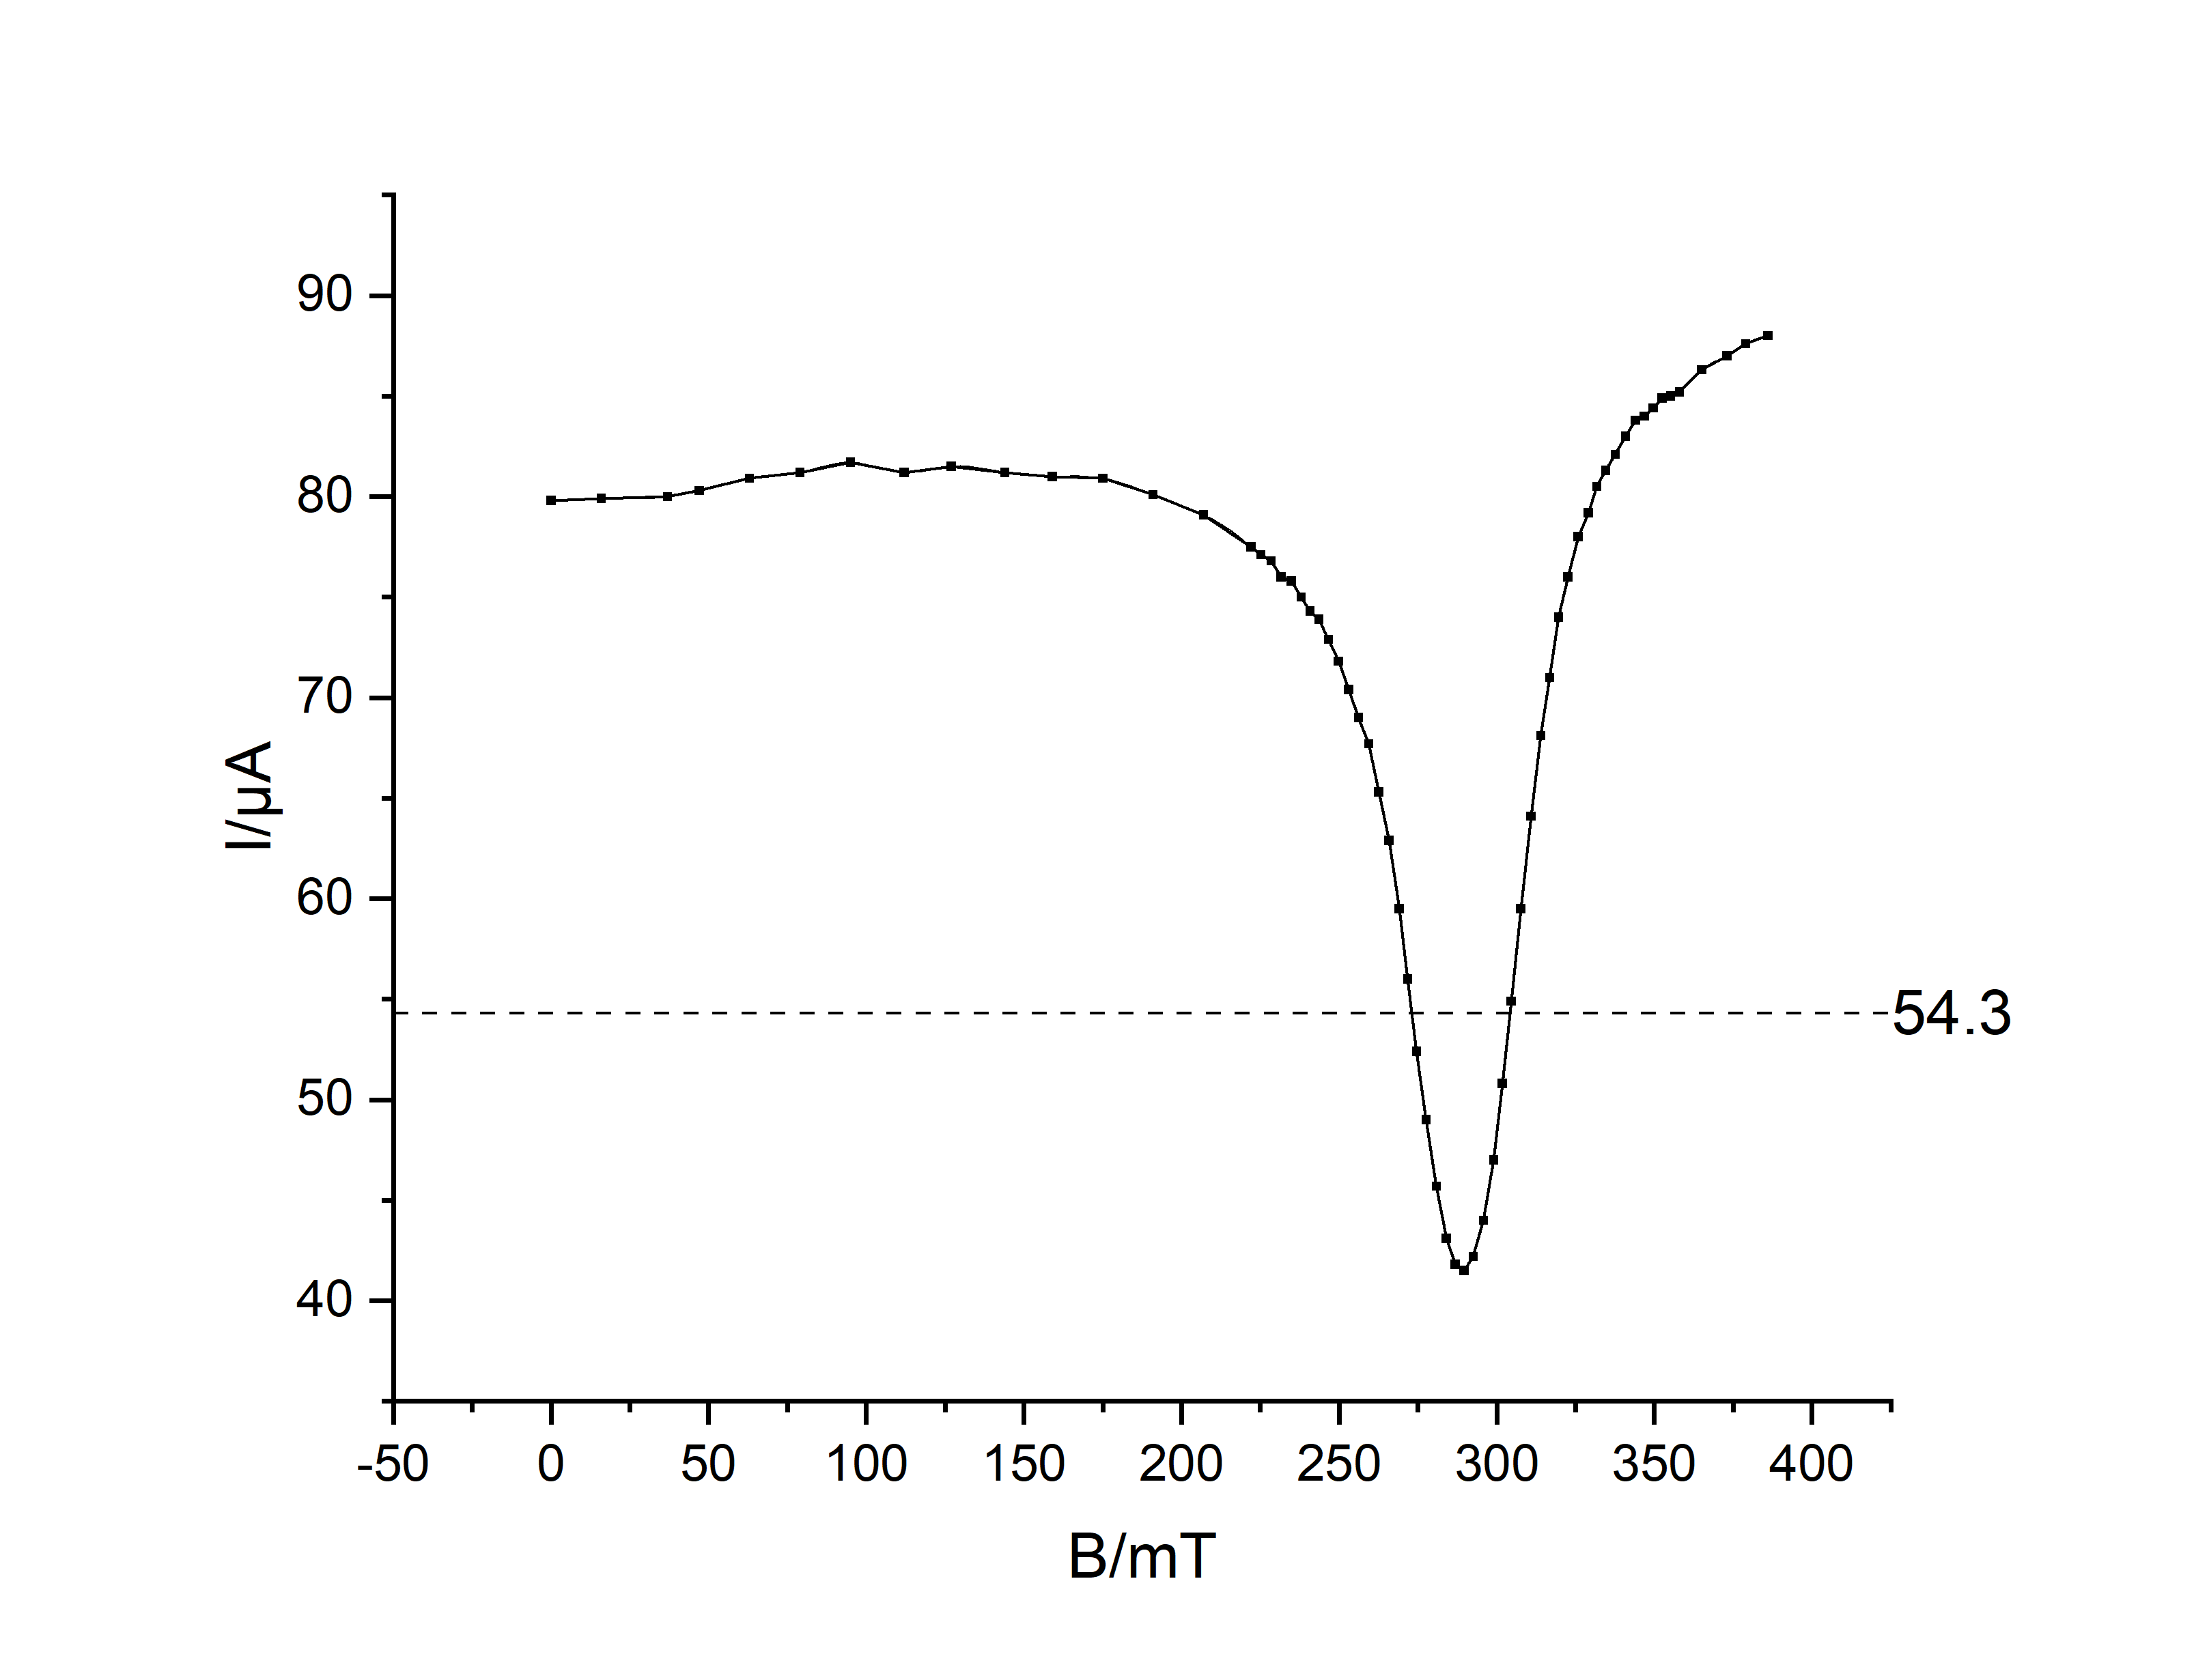
\includegraphics[scale=0.25]{Graph3.png}
	\caption{I-B图}
\end{figure}

从origin软件中得到近似得到最低点$I_r=41.5{\mu}A$

再通过非共振区域的平均值来得到合适的$I_0=82.1\mu{A}$

从而得到:
$$
I_{1/2}=\frac{2I_0I_r}{I_0+I_r}=\frac{2\times41.5\times82.1}{41.5+82.1}\mu{A}=54.3\mu{A}
$$

从图中我们还可以得到:
$$B_{r1} = 289.6mT$$
$$g = \frac{\gamma{h}}{2\pi\mu_B} = \frac{\omega{h}}{2\pi B_r \mu_B} = 3.52 \times 10^{-2} kg \cdot T^{-1} \cdot A^{-1}\cdot m^{-1}\cdot s^{-1}$$
$$ \Delta B_1 = 304.6 - 273.4 mT = 31.2 mT $$

我们再次从表中得到反向的磁感应强度,并绘制出一条$I-B$曲线:
\begin{figure}[htb]
	\centering
	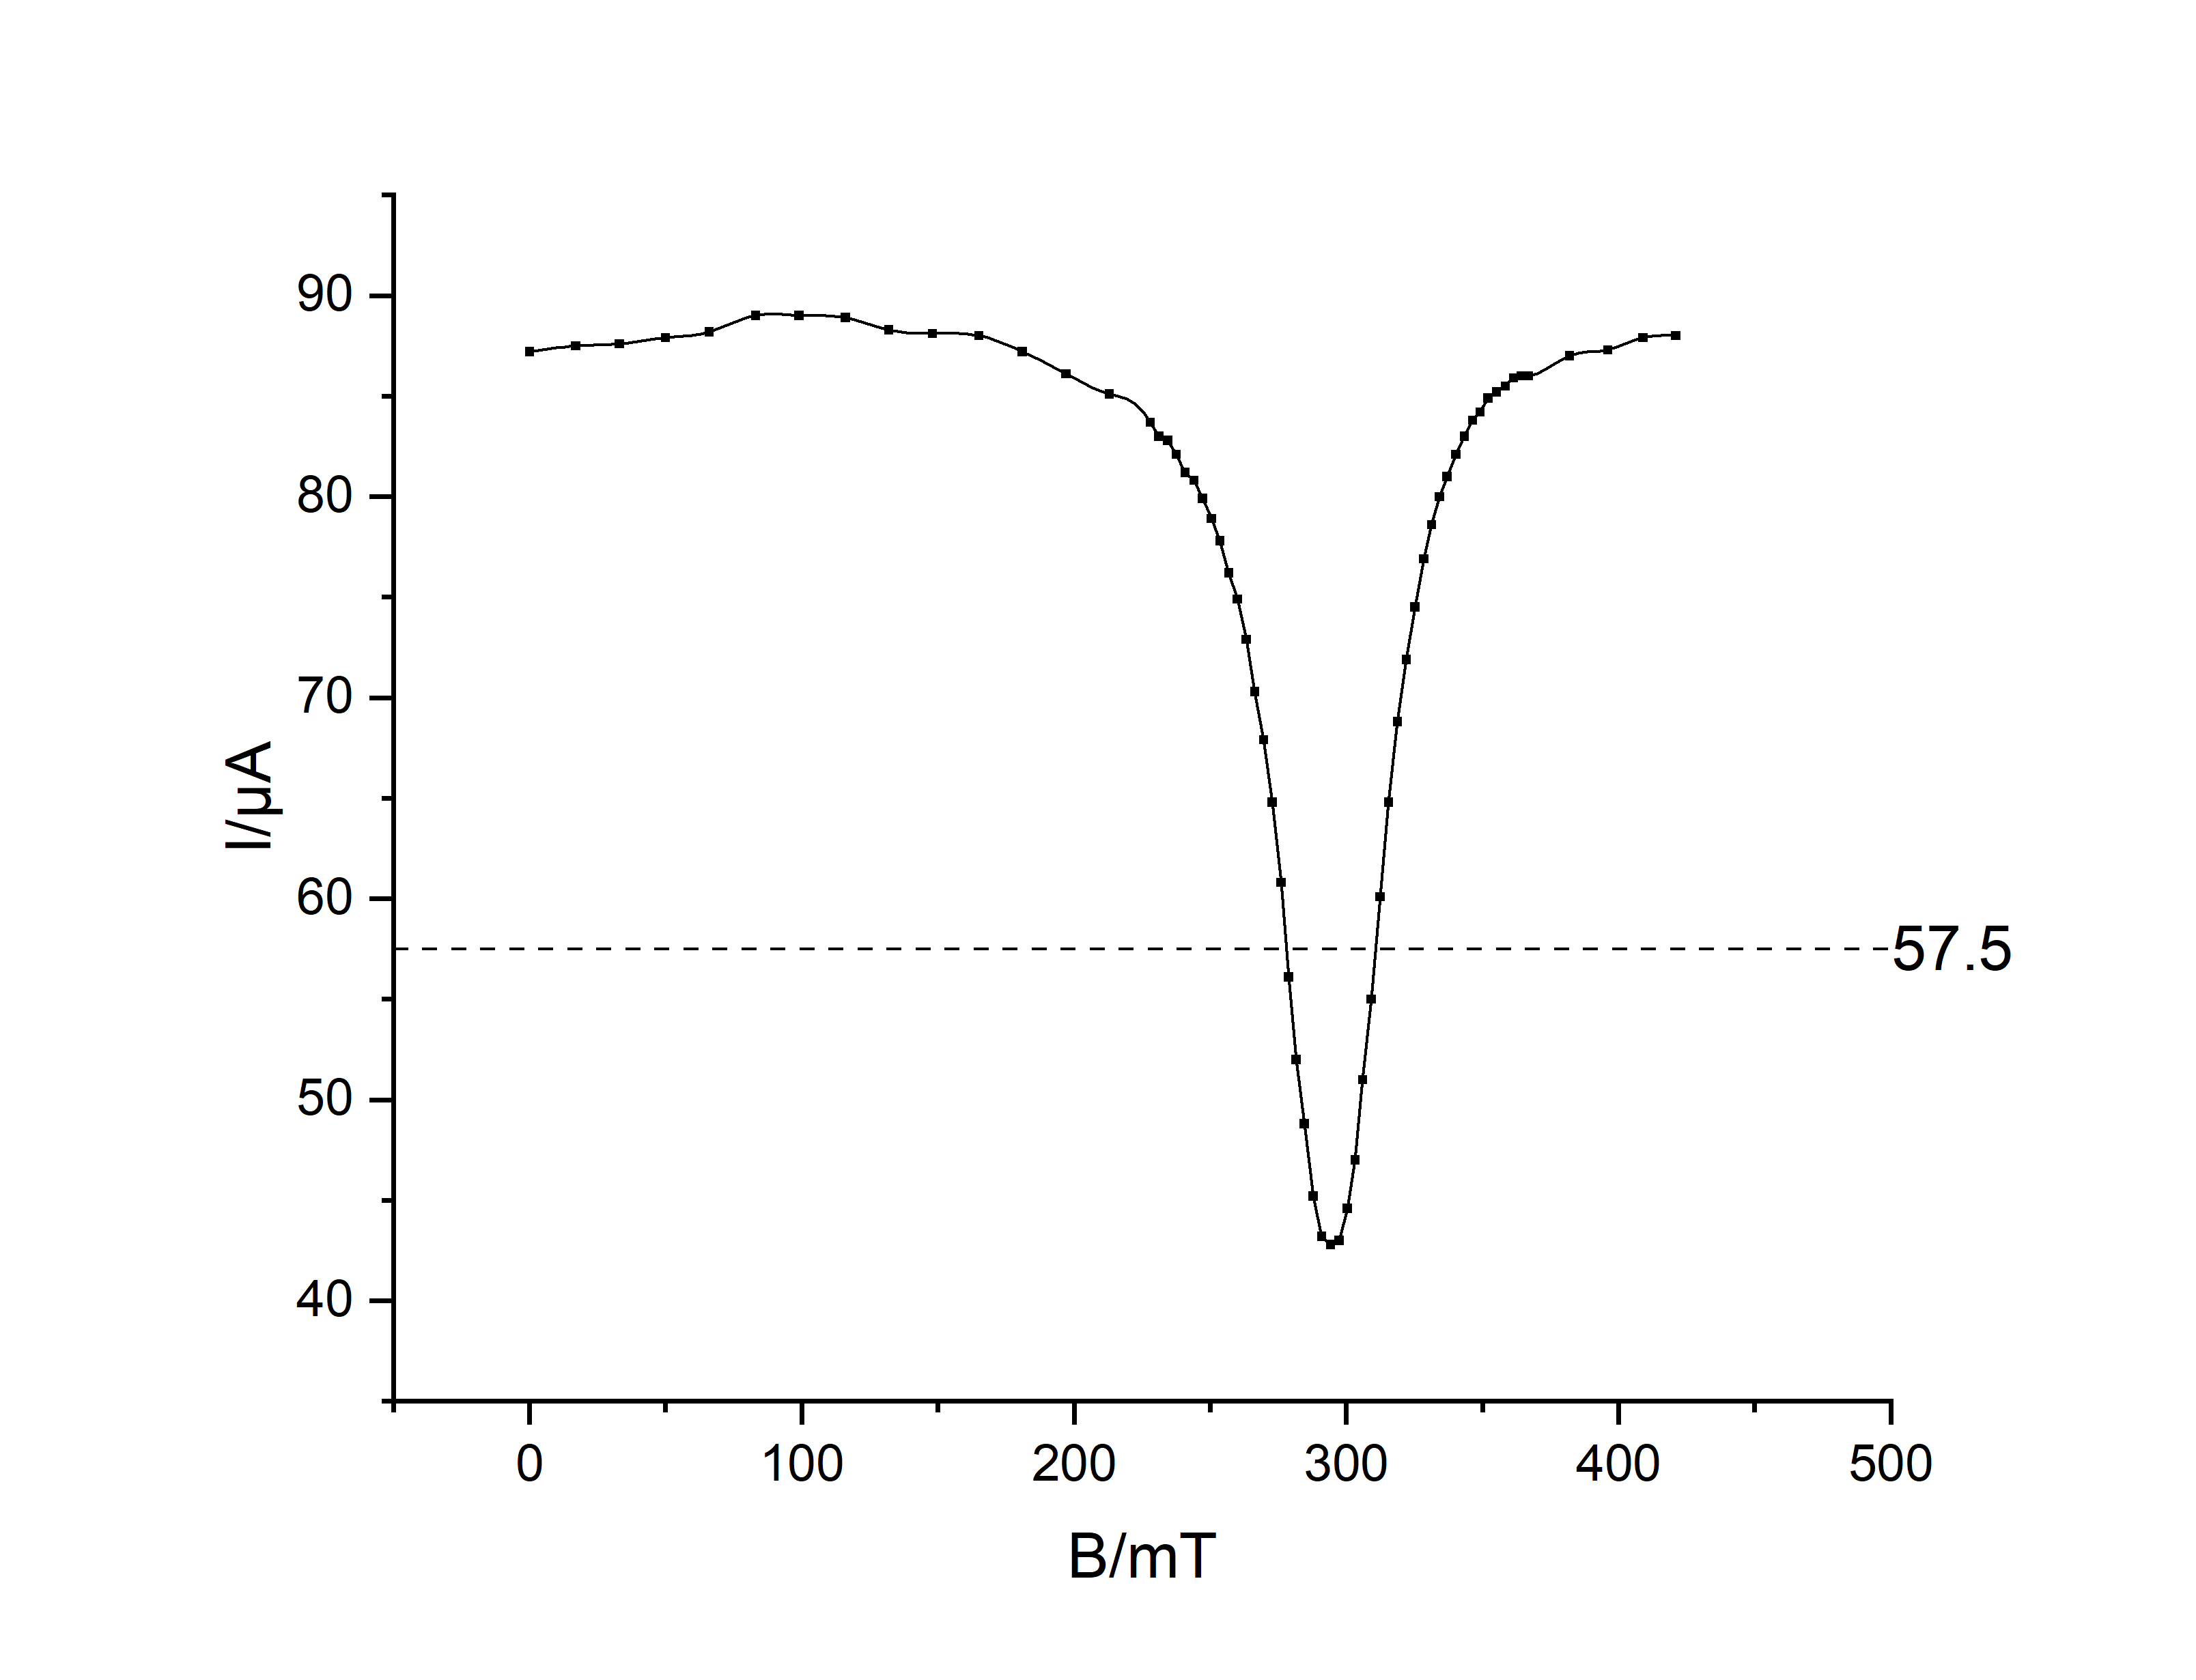
\includegraphics[scale=0.33]{Graph5.png}
	\caption{I-B图}
\end{figure}

最低点$I_r = 42.8 \mu A$

通过非共振区电流的平均值计算出$I_0 = 87.6 \mu A $

从而得到:
$$
I_{1/2}=\frac{2I_0I_r}{I_0+I_r}=\frac{2\times87.6\times42.8}{42.8+87.6}\mu A = 57.5\mu A
$$

从图中还可以得到:
$$B_{r1} = 294.2 mT $$
$$ \Delta B_2 = 311.2 - 278.4 mT = 32.8 mT $$

直接测量得出的共振电流为:
$$I = 1.855 A$$

查表对应的磁场为:
$$B_1 = 291 mT $$
$$B_2 = 299 mT $$

误差很小。

\subsection{观察共振波形}

我们再看看磁场电流达共振点值的示波器波形:
\begin{figure}[htb]
	\centering
	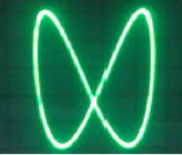
\includegraphics[scale=0.33]{1.png}
	\caption{示波器波形}
\end{figure}

我们从$y$方向上观察,没有扫描时,是一个$V$字形状的波。再调为$X-Y$图像,则在$X$方向上不断扫描,形成了如图所示的形状。

\subsection{思考题}

不能取一半高度处的$I$c处的磁场差,应该使用$I_{1/2} = \frac{2\times I_r I_0}{I_r + I_0}$公式计算,两个值并不相等。



\end{document}